% !TeX spellcheck = en_GB

\documentclass[10pt,xcolor=pdftex,dvipsnames,table]{beamer}

\usetheme{Boadilla}

\usepackage{lmodern}
\usepackage[T1]{fontenc}     % caracteres accentues
\usepackage[utf8]{inputenc}  %  encodage unicode des sources .tex
\usepackage{amsmath,amssymb,amsbsy,dsfont}

% pour \mybox...
\usepackage{xcolor}
\setlength{\fboxrule}{0.1pt}
\newcommand{\mybox}[2]{\fcolorbox{#1}{white}{$\displaystyle#2$}}


\title{Boundary Element Method}
\author{ MATH-0471 }
%\institute{University of Li\`ege}
\date{\today}

%\AtBeginSection[]
%{
%	\begin{frame}
%		\frametitle{Outline}
%		\tableofcontents[currentsection]
%	\end{frame}
%}


\begin{document}

\frame{\titlepage}

%\section*{Outline}

%\begin{frame}
%	\frametitle{Outline}
%	\tableofcontents
%\end{frame}

% ---------------------------------------------------------------------------------------
%\section{ FEM for 2D Linear Elasticity  }
% ---------------------------------------------------------------------------------------
\begin{frame}
	\frametitle{ Boundary Element Method }
	\framesubtitle{ Potential problem }
	
	\textbf{Potential problem} in $\Omega$:
	
	\begin{equation*}
		\left\{
		\begin{aligned}
		 &\Delta u = 0 &&\text{ in } \Omega  &&  \\
		&u = \bar{u} && \text{ on } \Gamma_D && \text{ (Dirichlet)}\\
		&\frac{\partial u}{\partial \boldsymbol{n}} = \bar{u}_n && \text{ on } \Gamma_N && \text{ (Neumann)} \\
		\end{aligned}
	\right.
	\end{equation*}
	
where 
\begin{itemize}
	\item $u$ is the scalar unknown, 
	\item $\Gamma$ is the boundary of $\Omega$ and $\Gamma_D \cup \Gamma_N = \Gamma$ and $\Gamma_D \cap \Gamma_N = \emptyset$,
	\item $\frac{\partial u}{\partial \boldsymbol{n}} = \boldsymbol{\nabla} u \cdot \boldsymbol{n}$, where $\boldsymbol{n}$ is the outward normal to $\Omega$.
\end{itemize}	
	\vspace{\stretch{1}}

Note that the PDE is homogeneous but the boundary conditions are not.
	\vspace{\stretch{1}}
	
	We follow here the notations from the book of \cite{Katsikadelis2016}, which is freely available from the \href{https://explore.lib.uliege.be/discovery/fulldisplay?docid=alma9919484598002321&context=L&vid=32ULG_INST:ULIEGE&lang=fr&search_scope=ULIEGE&adaptor=Local}{\color{blue}ULiege library website} (use VPN).

\end{frame}

\begin{frame}
	\frametitle{ Boundary Element Method }
	\framesubtitle{ Potential problem }
	
	\centerline{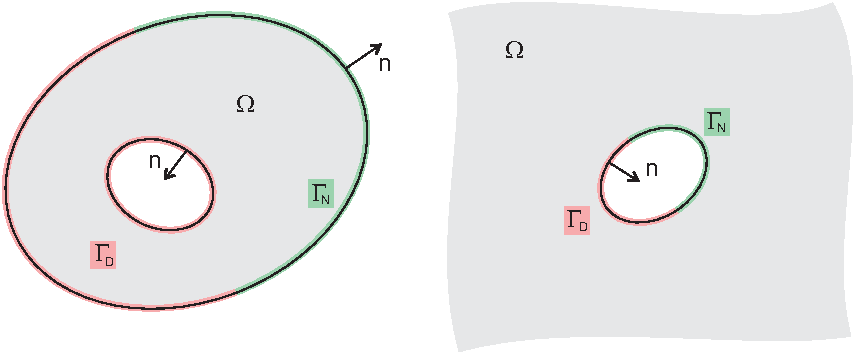
\includegraphics[width=\textwidth]{fig_domain}}	
		\vspace{\stretch{1}}
	The domain can be finite (left) or infinite (right).
\end{frame}

\begin{frame}
	\frametitle{ Boundary Element Method }
	\framesubtitle{ Fundamental solution / Free space Green's function in 2D}
	
	If we ignore the boundary conditions, a \textbf{fundamental solution} $v$ of the Laplace problem defined in $\mathds{R}^2$ can be found by solving the PDE with a Dirac impulse as right-hand side.
	
	\begin{equation*}
		\Delta v = \delta(\boldsymbol{Q}-\boldsymbol{P})
	\end{equation*}
	where $\boldsymbol{P} = \boldsymbol{P}(x,y)$ is the position of the Dirac impulse and $\boldsymbol{Q} = \boldsymbol{Q}(\xi,\eta)$ is the position where $v$ is evaluated
	
	\vspace{\stretch{1}}
	We obtain
	\begin{equation*}
		v(\boldsymbol{Q}, \boldsymbol{P}) = \frac{1}{2\pi}\ln r
	\end{equation*}	

	with $r = \sqrt{(\xi-x)^2+(\eta-y)^2} = || \boldsymbol{Q}-\boldsymbol{P} ||$
	
		\vspace{\stretch{1}}
		
	The fundamental solution is singular at $\boldsymbol{Q}=\boldsymbol{P}$.
	
\end{frame}










\begin{frame}
	\frametitle{ Boundary Element Method }
	\framesubtitle{ Representation formula in the domain $\Omega$ }
	
	\textbf{Green's second identity} (also called Green's reciprocal identity):
	
	\begin{equation*}
		\int_{\Omega} \left( v\,\Delta u - u\,\Delta v\, \right) d\Omega 
		=
		\int_{\Gamma} \left( v \frac{\partial u}{\partial \boldsymbol{n}} - u \frac{\partial v}{\partial \boldsymbol{n}} \right)\, ds
	\end{equation*}
	
	
	
	\vspace{\stretch{1}}
	
	From this equality, if we choose $v$ as the fundamental solution introduced earlier, we can write a \textbf{representation formula} for the solution $u$ of the Laplace equation in $\Omega$ (boundary excluded):
	
	\begin{equation*}
		u(\boldsymbol{P}) = - \int_{\Gamma} \left( v(\boldsymbol{P},\boldsymbol{q}) \frac{\partial u(\boldsymbol{q})}{\partial \boldsymbol{n}_q} - u(\boldsymbol{q}) \frac{\partial v(\boldsymbol{P},\boldsymbol{q})}{\partial \boldsymbol{n}_q} \right)\, ds_q
	\end{equation*}	
	
	\vspace{\stretch{1}}	
	
	Important remark concerning the notations:
	\begin{itemize}
		\item A capital letter $(\boldsymbol{P}, \boldsymbol{Q})$ represents a point inside the domain $\Omega$,
		\item A lowercase letter $(\boldsymbol{p},\boldsymbol{q})$ represents a point on the boundary of $\Omega$.
	\end{itemize}
	
	\vspace{\stretch{1}}	
	This formula can be used to compute $u$ in $\Omega$ if we know both $u(\boldsymbol{q})$ and $\frac{\partial u(\boldsymbol{q})}{\partial \boldsymbol{n}_q}$ on the boundary (but we don't: we have either one or the other).
	
\end{frame}


\begin{frame}
	\frametitle{ Boundary Element Method }
	\framesubtitle{ Representation formula on the boundary $\Gamma$ }
	
	From the Green's second identity, it is also possible to deduce a representation formula for the solution $u$ lying on $\Gamma$:
	
	\begin{equation*}
		\frac{\alpha}{2\pi} u(\boldsymbol{p}) = - \int_{\Gamma} \left( v(\boldsymbol{p},\boldsymbol{q}) \frac{\partial u(\boldsymbol{q})}{\partial 	\boldsymbol{n}_q} - u(\boldsymbol{q}) \frac{\partial v(\boldsymbol{p},\boldsymbol{q})}{\partial \boldsymbol{n}_q} \right)\, ds_q
	\end{equation*}		
	
	where $\alpha$ is the angle of the corner made by the boundary at $\boldsymbol{p}$.
	
	\vspace{\stretch{1}}	
	\centerline{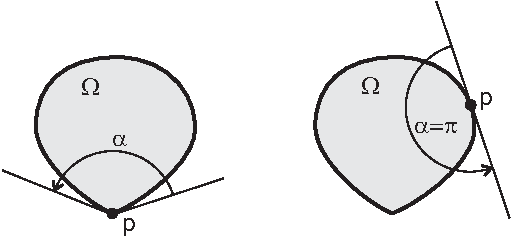
\includegraphics[width=0.5\textwidth]{fig_alpha}}	
		
	If the boundary is smooth, $\alpha=\pi$ and the coefficient in front of $u(\boldsymbol{p})$ is $\frac{1}{2}$.
	
	\vspace{\stretch{1}}	
	This \textbf{boundary integral equation} can be used to calculate $u$ and its derivative on the boundary.
	
\end{frame}


\begin{frame}
	\frametitle{ Boundary Element Method }
	\framesubtitle{ Principle of the BEM }
	
	\begin{itemize}
	\item The Boundary Element Method consists in meshing the boundary of the problem with a series of $N$ ``boundary elements''. 
	\item On each element, the solution $u$ is approximated by simple polynomials  (constant, linear, etc.).
	\item Injecting this approximation into the boundary integral equation and taking into account the boundary conditions allows us to calculate the solution and its derivative on the whole boundary.
	\item Eventually, the solution inside the domain can be computed from the values on the boundary with the help of the representation formula.
	\end{itemize}
	
\end{frame}



\begin{frame}
	\frametitle{ Boundary Element Method }
	\framesubtitle{ Constant boundary elements }
	
	\begin{itemize}
		\item The simplest way to approximate the solution is to use a piecewise-linear approximation of the boundary (a series of oriented straight segments).
	
		\item On each element the solution $u$ and its derivative $u_n$ is considered constant (thus discontinuous across elements). 
	
		\item We also define a node at the centre of each segment.
	\end{itemize}	

	\vspace{\stretch{1}}	
	\centerline{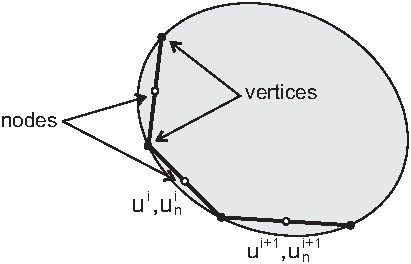
\includegraphics[width=0.4\textwidth]{fig_mesh}}	

\end{frame}



\begin{frame}
	\frametitle{ Boundary Element Method }
	\framesubtitle{ Solving the boundary }
	
	Discretized Boundary Integral Equation:
	\begin{equation*}
		\frac{1}{2} u_i = - \sum_{j=1}^{N} \int_{\Gamma_j} v(\boldsymbol{p}_i, \boldsymbol{q}) 
		\underbrace{ \frac{\partial u(\boldsymbol{q})}{\partial \boldsymbol{n}_q} }_{u_n^j}   
		\,ds_q
		+ \sum_{j=1}^{N} \int_{\Gamma_j} 
		\underbrace{u(\boldsymbol{q})}_{u^j} 
		\frac{\partial v(\boldsymbol{p}_i,\boldsymbol{q})}{\partial \boldsymbol{n}_q}\,ds_q
	\end{equation*}		
	
	Thanks to the node position centred in the middle of each segment, the boundary is locally smooth and $\alpha=\frac{1}{2}$.

			\vspace{\stretch{1}}	
			
	Reordering the terms:
	\begin{equation*}
		-\frac{1}{2} u^i 
			+ \sum_{j=1}^{N}
			\underbrace{ 
	    \left[\int_{\Gamma_j} \frac{\partial v(\boldsymbol{p}_i,\boldsymbol{q})}{\partial \boldsymbol{n}_q}\,ds_q\right] 
			}_{\hat{H}_{ij}}
		 u^j
		= \sum_{j=1}^{N} 
			\underbrace{ 	
		\left[ \int_{\Gamma_j} v(\boldsymbol{p}_i, \boldsymbol{q}) \,ds_q   \right] 
		    		}_{G_{ij}}
		  u_n^j
	\end{equation*}	

\end{frame}



\begin{frame}
	\frametitle{ Boundary Element Method }
	\framesubtitle{ Solving the boundary }
	
	\begin{equation*}
		\sum_{j=1}^{N}
		H_{ij}
		u^j
		= \sum_{j=1}^{N} 
		G_{ij}
		u_n^j
		\qquad
		\text{ with }
		\left\{
		\begin{aligned}
			&H_{ij} = \int_{\Gamma_j} \frac{\partial v(\boldsymbol{p}_i,\boldsymbol{q})}{\partial \boldsymbol{n}_q}\,ds_q -\frac{1}{2}\delta_{ij} \\
			&G_{ij} =  \int_{\Gamma_j} v(\boldsymbol{p}_i, \boldsymbol{q}) \,ds_q 
		\end{aligned}
		\right.
	\end{equation*}	
	
	%\vspace{\stretch{1}}	
	\centerline{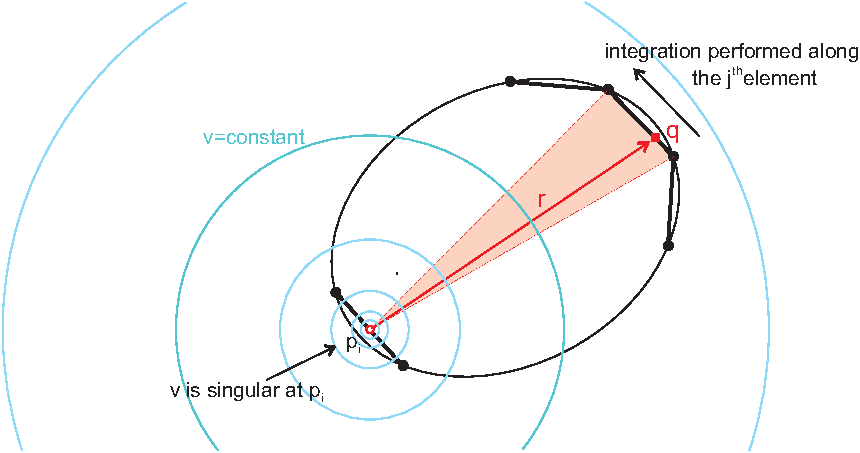
\includegraphics[width=0.75\textwidth]{fig_integration}}	

	Difficulties are expected when $i=j$ (singular integrand).
\end{frame}


\begin{frame}
	\frametitle{ Boundary Element Method }
	\framesubtitle{ Solving the boundary }
	
	In matrix form
	\begin{equation*}
		[H] \{u\} = [G] \{u_n\}
	\end{equation*}	
	
	Equations can be sorted according to the type of boundary condition  prescribed at the corresponding node (e.g. Dirichlet first, then Neumann):

	\begin{equation*}
		\begin{bmatrix}
			\qquad\\
			[H_{D}] & [H_N] \\
			\qquad\\
		\end{bmatrix}
		\begin{Bmatrix}
			\{u\}_D \\
			\{u\}_N \\
		\end{Bmatrix}
		=
		\begin{bmatrix}
			\qquad\\
			[G_{D}] & [G_N] \\
			\qquad\\
		\end{bmatrix}
		\begin{Bmatrix}
			\{u_n\}_D \\
			\{u_n\}_N \\
		\end{Bmatrix}
	\end{equation*}	
	Since $\{u\}_D = \{\bar{u}\}$ and $\{u_n\}_N  = \{\bar{u}_n\}$, we can gather the unknowns in the left-hand side:

	\begin{equation*}
	\underbrace{
	\begin{bmatrix}
		\qquad\\
		[H_N] & -[G_D] \\
		\qquad\\
	\end{bmatrix}
}_{[A]}
	\underbrace{
	\begin{Bmatrix}
		\{u\}_N \\
		\{u_n\}_D \\
	\end{Bmatrix}
}_{\{x\}}
	=
	\underbrace{
	\begin{bmatrix}
		\qquad\\
		-[H_{D}] & [G_N] \\
		\qquad\\
	\end{bmatrix}
	\begin{Bmatrix}
		\{\bar{u}\} \\
		\{\bar{u}_n\} \\
	\end{Bmatrix}
}_{ \{b\}}
\end{equation*}	
This system is then solved using a linear solver.	
	
\end{frame}



\begin{frame}
	\frametitle{ Boundary Element Method }
	\framesubtitle{ Calculation of $[G]$ }
	
	$\bullet$ $G_{ij}$ with $i\neq j$ (Gauss quadrature): 
	\begin{equation*}
		G_{ij} =  \int_{\Gamma_j} v(\boldsymbol{p}_i, \boldsymbol{q}) \,ds_q = \int_{-1}^1 \frac{1}{2\pi} \ln (r(\xi))\,\frac{l_j}{2}\,d\xi 
		= \frac{l_j}{4\pi} \sum_{k=1}^{N^{GP}} \ln (r(\xi_k))\, w_k
	\end{equation*}		
	where $l_j$ is the length of element $j$ and $N^{GP}$ is the number of Gauss points with are located at $\xi_k$ with weight $w_k$.
	
	\vspace{\stretch{1}}	
	
	$\bullet$ $G_{ii}$ (analytical integration):
	\begin{equation*}
	G_{ii} =  \frac{l_i}{2\pi} \left( \ln\frac{l_i}{2}-1\right)
\end{equation*}	

\end{frame}


\begin{frame}
	\frametitle{ Boundary Element Method }
	\framesubtitle{ Calculation of $[H]$ }
	
	$\bullet$ $H_{ij}$ with $i\neq j$ (analytical integration): 
	\begin{equation*}
		H_{ij} =  \int_{\Gamma_j} \frac{\partial v(\boldsymbol{p}_i,\boldsymbol{q})}{\partial \boldsymbol{n}_q}\,ds_q
		= \frac{a_{j+1}-a_j}{2\pi}
	\end{equation*}		

	%\vspace{\stretch{1}}	
	\centerline{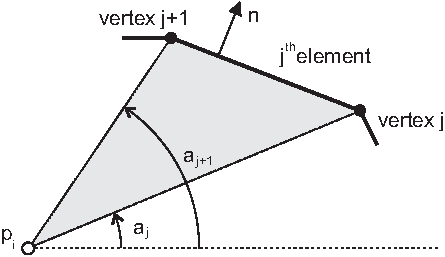
\includegraphics[width=0.45\textwidth]{fig_hij}}		
	
	\vspace{\stretch{1}}	
	
	$\bullet$ $H_{ii}$ (analytical integration):
	\begin{equation*}
		\hat{H}_{ii} = 0 \qquad \Rightarrow
		H_{ii} = -\frac{1}{2}
	\end{equation*}	
	
\end{frame}


\begin{frame}
	\frametitle{ Boundary Element Method }
	\framesubtitle{ Calculation of the solution inside $\Omega$ }
	
	From the representation formula:
	\begin{equation*}
		u(\boldsymbol{P}) = - \int_{\Gamma} \left( v(\boldsymbol{P},\boldsymbol{q}) \frac{\partial u(\boldsymbol{q})}{\partial \boldsymbol{n}_q} - u(\boldsymbol{q}) \frac{\partial v(\boldsymbol{P},\boldsymbol{q})}{\partial \boldsymbol{n}_q} \right)\, ds_q
	\end{equation*}	

	we can write:
	\begin{equation*}
	u(\boldsymbol{P}) = -\sum_{j=1}^{N} 
		\left[ \int_{\Gamma_j} v(\boldsymbol{P}, \boldsymbol{q}) \,ds_q   \right] 
	u_n^j
	+ \sum_{j=1}^{N} 
		\left[\int_{\Gamma_j} \frac{\partial v(\boldsymbol{P},\boldsymbol{q})}{\partial \boldsymbol{n}_q}\,ds_q\right] 
	u^j
\end{equation*}	

\begin{itemize}
	\item The solution inside $\Omega$ requires the computation of boundary integrals with regular integrands (the singularity is located at $\boldsymbol{P}$). Refer to the expressions of $H_{ij}$ and $G_{ij}$ for $i\neq j$. 
	\item If the solution at several points need to be computed, it can be easily performed in parallel.
\end{itemize}
	
	
\end{frame}



\begin{frame}
	\frametitle{ Boundary Element Method }
	\framesubtitle{ Summary }
	
	Advantages of the BEM:
	\begin{itemize}
		\item Only the surface of the problem should be meshed (the problem dimension is decreased by 1 compared to FEM).
		\item The domain can be infinite.
		\item The solution and its derivative can be easily evaluated anywhere in the domain.
		\item Works well for stationary, linear and homogeneous PDEs with non-homogeneous boundary conditions.
	\end{itemize}
	
	\vspace{\stretch{1}}		
	
	Typical applications:
	\begin{itemize}
		\item Potential problems: stationary heat conduction, electrostatics, irrotational flows, Darcy flows,
		\item Acoustics (Helmholtz equation),
		\item Slow viscous flows (Stokes equations),
		\item Elasticity (Lamé equations).
	\end{itemize}

\end{frame}



\begin{frame}
	\frametitle{ Boundary Element Method }
	\framesubtitle{ Summary }
	
	Issues of the BEM:
	\begin{itemize}
		\item The method requires an \textbf{integral representation} of the solution and a fundamental solution to be calculated, which is sometimes impossible (e.g. nonlinear equations).
		\item Integrals of \textbf{singular functions} must be evaluated very precisely with special techniques for obtaining accurate results.
		\item The method relies on \textbf{non-sparse, non-symmetric matrices} which lead large memory requirement and CPU time. Thus, complicated acceleration techniques (fast multipole method, hierarchical matrices) are needed for 3D problems.
	\end{itemize}
\end{frame}

%------------------------------------------------

\begin{frame}
	\frametitle{References}
	\footnotesize{
		\begin{thebibliography}{99} % Beamer does not support BibTeX so references must be inserted manually as below
			\bibitem[Katsikadelis, 2016]{Katsikadelis2016} John T. Katsikadelis (2016)
			\newblock The Boundary Element Method for Engineers and Scientists -- Theory and Applications
			\newblock Elsevier, \emph{Second edition}, ISBN: 9780128044933
		\end{thebibliography}
	}
\end{frame}


\end{document}
